% !TeX program = pdflatex
% !BIB program = biber
% ================================================================
% BESONDERE LERNLEISTUNG (BLL) – VORLAGE FUER HESSEN / SFN
% EINSTIEG: 1) angaben.tex bearbeiten 2) kapitel/*.tex anpassen
%          3) bll.tex kompilieren (LaTeX -> Biber -> LaTeX x2)
% ================================================================
\documentclass[12pt,a4paper,oneside,headings=normal,numbers=noenddot,
               parskip=half,listof=totoc]{scrreprt}

% ================================================================
% BLL-VORLAGE: HIER ALLE PERSONEN- UND SCHULDATEN EINTRAGEN
% ================================================================
% Alles in geschweiften Klammern darf geändert werden.
% Bitte die Beispielfelder vor Abgabe vollständig ersetzen!

\newcommand{\Arbeitstitel}{Untersuchung der Schwingungsdauer eines Fadenpendels}
\newcommand{\Untertitel}{Theoretische Grundlagen und Konzept einer experimentellen Prüfung}
\newcommand{\Kurztitel}{Schwingungsdauer eines Fadenpendels}

\newcommand{\Autor}{Vorname Nachname}
\newcommand{\Schule}{Name der Schule}
\newcommand{\Schulort}{Kassel}
\newcommand{\Jahrgang}{Qualifikationsphase Q3/Q4}
\newcommand{\KlasseOderKurs}{Physik (Referenzfach)}
\newcommand{\Abiturjahr}{2027}
\newcommand{\BetreuungSchule}{Name der betreuenden Lehrkraft}
\newcommand{\Abgabedatum}{TT. Monat JJJJ}

% Externe Begleitung ist optional und KEINE schulische Prüfungsfunktion.
% Wenn keine externe Betreuung besteht: \MitSFNfalse setzen.
\newif\ifMitSFN
\MitSFNtrue
\newcommand{\ExterneEinrichtung}{Schülerforschungszentrum Nordhessen (SFN)}
\newcommand{\BetreuungSFN}{Name der fachlichen Ansprechperson}

% Falls die Schule keinen abstrakten Text / keine Verzeichnisse verlangt,
% die betreffenden \input-Zeilen in bll.tex entfernen.
% Logos sind optional: logos/schule.pdf oder logos/schule.png
%                      logos/sfn.pdf oder logos/sfn.png

% ================================================================
% GESTALTUNG: möglichst nur die Angaben in angaben.tex ändern.
% Diese Einstellungen geben eine ruhige, wissenschaftliche Optik.
% ================================================================
\usepackage[T1]{fontenc}
\usepackage[utf8]{inputenc}
\usepackage[ngerman]{babel}
\usepackage{lmodern}
\usepackage{microtype}
\usepackage{setspace}
\onehalfspacing
\usepackage[left=3.2cm,right=2.6cm,top=2.7cm,bottom=2.8cm,headsep=.7cm,head=22pt]{geometry}
\usepackage{graphicx}
\usepackage{amsmath,amssymb}
\usepackage{siunitx}
\sisetup{locale=DE,per-mode=symbol,detect-all}
\usepackage{booktabs}
\usepackage{tabularx}
\usepackage{csquotes}
\usepackage{listings} % optionaler Programmcode-Anhang
\usepackage{xcolor}
\definecolor{BLLblau}{HTML}{243C54}
\definecolor{BLLgrau}{HTML}{65717B}
\usepackage[font=small,labelfont=bf]{caption}
\usepackage{scrlayer-scrpage}
\setlength{\footheight}{22pt}
\clearpairofpagestyles
\automark[chapter]{chapter}
\ihead{\headmark}
\ohead{}
\cfoot[\pagemark]{\pagemark}
\setkomafont{pagehead}{\small\normalfont\color{BLLgrau}}
\setkomafont{pagefoot}{\small\normalfont\color{BLLgrau}}
\setkomafont{chapter}{\Large\bfseries\color{BLLblau}}
\setkomafont{section}{\large\bfseries\color{BLLblau}}
\setkomafont{subsection}{\normalsize\bfseries}
\KOMAoptions{headsepline=0.35pt}
\setlength{\emergencystretch}{2em}
\usepackage[backend=biber,style=authoryear,sorting=nyt,maxcitenames=2]{biblatex}
\addbibresource{literatur.bib}
\usepackage[hidelinks,unicode]{hyperref}
\hypersetup{pdftitle={\Arbeitstitel},pdfauthor={\Autor},pdfsubject={Besondere Lernleistung}}

% Gibt automatisch zuerst das Schul- oder SFN-Logo aus, falls vorhanden.
% Niemals ein Logo ohne Genehmigung verwenden.
\newcommand{\SchulLogo}{%
  \IfFileExists{logos/schule.pdf}{\includegraphics[height=1.45cm,keepaspectratio]{logos/schule.pdf}}{%
    \IfFileExists{logos/schule.png}{\includegraphics[height=1.45cm,keepaspectratio]{logos/schule.png}}{\textcolor{BLLgrau}{\small\sffamily\bfseries\Schule}}}}
\newcommand{\SFNLogo}{%
  \IfFileExists{logos/sfn.pdf}{\includegraphics[height=1.45cm,keepaspectratio]{logos/sfn.pdf}}{%
    \IfFileExists{logos/sfn.png}{\includegraphics[height=1.45cm,keepaspectratio]{logos/sfn.png}}{\textcolor{BLLgrau}{\small\sffamily SFN \textbar\ Nordhessen}}}}


\begin{document}
\hypersetup{pageanchor=false}
% Selbst gestaltete, bewusst zurückhaltende Titelseite.
% Achtung: eine offizielle schulische Titelseitenvorgabe hat Vorrang.
\begin{titlepage}
  \thispagestyle{empty}
  \setstretch{1.12}
  \noindent
  \begin{minipage}[c]{.57\textwidth}
    \SchulLogo
  \end{minipage}
  \begin{minipage}[c]{.38\textwidth}
    \ifMitSFN\raggedleft\SFNLogo\fi
  \end{minipage}

  \vspace*{1.9cm}
  \noindent{\small\sffamily\bfseries\color{BLLgrau}
    BESONDERE LERNLEISTUNG \quad | \quad ABITUR \Abiturjahr\par}
  \vspace{.3cm}
  \noindent\textcolor{BLLblau}{\rule{\textwidth}{1.3pt}}
  \vspace{1.25cm}

  \noindent{\huge\bfseries\raggedright\hyphenpenalty=10000\exhyphenpenalty=10000\color{BLLblau}\Arbeitstitel\par}
  \vspace{.85cm}
  \noindent{\Large\color{BLLgrau}\Untertitel\par}
  \vfill

  \par\hrule height .3pt\vspace{.55cm}
  \noindent
  \begin{tabularx}{.97\textwidth}{@{}>{\bfseries}p{.38\textwidth}X@{}}
    Verfasser/in: & \Autor \\[.2cm]
    Schule: & \Schule, \Schulort \\[.2cm]
    Jahrgangsstufe: & \Jahrgang \\[.2cm]
    Referenzfach/Kurs: & \KlasseOderKurs \\[.2cm]
    Schulische Betreuung: & \BetreuungSchule \\[.2cm]
    \ifMitSFN SFN-Begleitung: & \BetreuungSFN\\
      & {\small\ExterneEinrichtung} \\[.2cm]\fi
    Abgabedatum: & \Abgabedatum \\[.55cm]
    \multicolumn{2}{@{}l@{}}{\small\color{BLLgrau} Schriftliche Ausarbeitung im Rahmen der besonderen Lernleistung}
  \end{tabularx}
\end{titlepage}
\setstretch{1.5}

\hypersetup{pageanchor=true}

%\pagenumbering{Roman}
\pagestyle{scrheadings}
\chapter*{Kurzfassung}
\addcontentsline{toc}{chapter}{Kurzfassung}
\markboth{Kurzfassung}{Kurzfassung}
% In einer echten Arbeit: 120–200 Wörter, je nach Schulvorgabe.
% Fragestellung, Methode, wichtigste Ergebnisse, Schlussfolgerung.
\textit{Hinweis zur Vorlage: Der folgende Text ist ein didaktisches
Beispiel. Er beschreibt keine tatsächlich durchgeführten Messungen.
Vor Abgabe muss er vollständig durch eine eigene Kurzfassung ersetzt werden.}

Diese Musterarbeit untersucht den Zusammenhang zwischen der Länge
\(l\) eines idealisierten Fadenpendels und seiner Schwingungsdauer
\(T\). Aus der Theorie des harmonischen Oszillators wird eine
Modellgleichung herangezogen. Anhand rechnerisch erzeugter Werte wird
gezeigt, wie sich wissenschaftliche Aussagen mit Tabellen, Abbildungen
und Quellen belegen lassen. Eine eigene Messreihe ist in dieser
Vorlage nicht enthalten. Eine tatsächliche besondere Lernleistung
müsste eine selbstständig durchgeführte Untersuchung sowie eine
kritische Bewertung der Beobachtungen dokumentieren.
\clearpage

\begingroup\singlespacing\small\tableofcontents\endgroup
% OPTIONAL: bei mehreren Abbildungen bzw. Tabellen aktivieren:
\listoffigures%
\listoftables%
\cleardoublepage
%\pagenumbering{arabic}

% HAUPTTEIL: Forschungsfrage -> Methode -> Befund -> Bewertung
\chapter{Einleitung}
\label{ch:einleitung}

\section{Problemstellung und Motivation}
% Ersetzen: Warum ist das Problem relevant? Wo ist die Forschungslücke?
Ein Fadenpendel ist ein einfaches physikalisches System, an dem sich
die Beziehung zwischen Modell und Beobachtung untersuchen lässt.
Die folgende Beispieldarstellung demonstriert die Struktur einer
wissenschaftlichen Arbeit, stellt aber selbst keine Forschungsleistung dar.

\section{Forschungsfrage und Hypothese}
% Die Forschungsfrage muss präzise und messbar bzw. prüfbar sein.
\textbf{Mögliche Forschungsfrage:} Wie hängt die Schwingungsdauer eines
Fadenpendels bei kleinen Auslenkwinkeln von der Pendellänge ab?

\textbf{Hypothese:} Unter idealisierten Bedingungen wächst die
Schwingungsdauer proportional zur Quadratwurzel der Pendellänge.

\section{Ziel und Aufbau der Arbeit}
In Kapitel~\ref{ch:theorie} werden die theoretischen Grundlagen
beschrieben, in Kapitel~\ref{ch:methodik} ein möglicher Versuchsablauf
skizziert. Kapitel~\ref{ch:ergebnisse} zeigt ausschließlich
\emph{berechnete Modellwerte}; ihre Grenzen werden in
Kapitel~\ref{ch:diskussion} diskutiert.

\chapter{Fachlicher Hintergrund und Forschungsstand}
\label{ch:theorie}

\section{Begriffe und theoretisches Modell}
Ein idealisiertes Fadenpendel besteht aus einer punktförmigen Masse,
die an einem masselosen Faden befestigt ist. Für kleine Auslenkungen
lässt sich die Schwingungsdauer näherungsweise durch
\begin{equation}
  \label{eq:pendel}
  T = 2\pi\sqrt{\frac{l}{g}}
\end{equation}
beschreiben. Dabei ist \(l\) die Pendellänge und \(g\) die lokale
Fallbeschleunigung. Diese Kleinwinkelnäherung und ihre Voraussetzungen
werden etwa bei \textcite{openstax-pendel} erläutert.

\section{Gültigkeitsbereich und offene Fragen}
Das Modell setzt unter anderem eine kleine Amplitude und vernachlässigbare
Reibung voraus. Eine tatsächliche Untersuchung sollte festlegen, ob
diese Voraussetzungen im Versuchsaufbau hinreichend erfüllt sind.
% In der echten BLL hier: Quellenvergleich, Begriffsdefinitionen,
% dokumentierter Forschungsstand und Begründung des eigenen Beitrags.

\chapter{Material und Methoden}
\label{ch:methodik}

\section{Versuchsaufbau}
Abbildung~\ref{fig:pendel} zeigt eine eigens erstellte schematische
Darstellung eines Fadenpendels. In einer echten Arbeit gehören hier
Fotos oder Skizzen des \emph{tatsächlich verwendeten} Aufbaus hinein.

\begin{figure}[htbp]
  \centering
  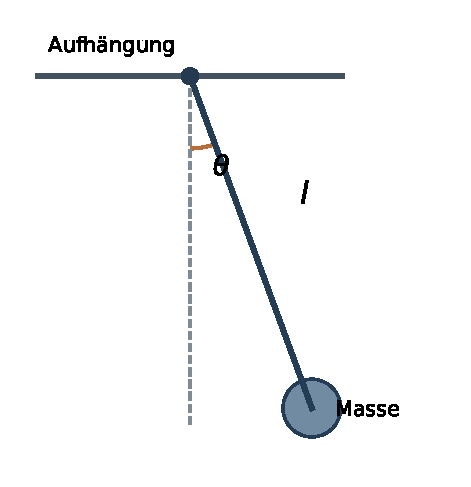
\includegraphics[width=.6\linewidth]{abbildungen/pendel-schema.pdf}
  \caption{Schematisches Fadenpendel (eigene Illustration für die Vorlage)}
  \label{fig:pendel}
\end{figure}

\section{Messverfahren und Dokumentation}
\textbf{Beispiel für eine mögliche Planung (nicht durchgeführt):}
Die Länge wird zwischen Aufhängepunkt und Schwerpunkt der Masse
bestimmt. Für mehrere Längen werden jeweils zehn Perioden zeitlich
erfasst. Die Zeit pro Periode ergibt sich aus der Division der
Gesamtmesszeit durch zehn. Jede Einstellung wird mehrfach wiederholt.

\section{Auswertung und Unsicherheiten}
Bei einer echten Messung müssen Gerätetypen, Kalibrierung,
Messwiederholungen und Unsicherheiten nachvollziehbar angegeben werden.
Eine mögliche Auswertungsgröße wäre \(T^2\), die nach
Gleichung~\eqref{eq:pendel} linear mit \(l\) zusammenhängt.
% WICHTIG: echte Rohdaten, Messprotokolle und Auswertungscode aufbewahren.

\chapter{Ergebnisse}
\label{ch:ergebnisse}

\section{Theoretische Modellwerte – keine Messdaten}
Die Werte in Tabelle~\ref{tab:modell} wurden allein mithilfe von
Gleichung~\eqref{eq:pendel} für \(g=\qty{9.81}{\meter\per\second\squared}\)
berechnet. \textbf{Es handelt sich ausdrücklich nicht um experimentell
gewonnene Daten.}

\begin{table}[htbp]
  \centering
  \caption{Rechnerisch erzeugte Demonstrationswerte; keine Messwerte}
  \label{tab:modell}
  \begin{tabular}{S[table-format=1.2] S[table-format=1.3]}
    \toprule
    {Pendellänge \(l\) (\si{\meter})} & {Modellperiode \(T\) (\si{\second})} \\
    \midrule
    0.25 & 1.003 \\
    0.50 & 1.419 \\
    0.75 & 1.737 \\
    1.00 & 2.006 \\
    \bottomrule
  \end{tabular}
\end{table}

\section{Grafische Darstellung}
Abbildung~\ref{fig:modell} veranschaulicht denselben berechneten
Zusammenhang. In einer echten BLL sollten hier eigene Messergebnisse,
Fehlerbalken und gegebenenfalls ein Modellvergleich stehen.

\begin{figure}[htbp]
  \centering
  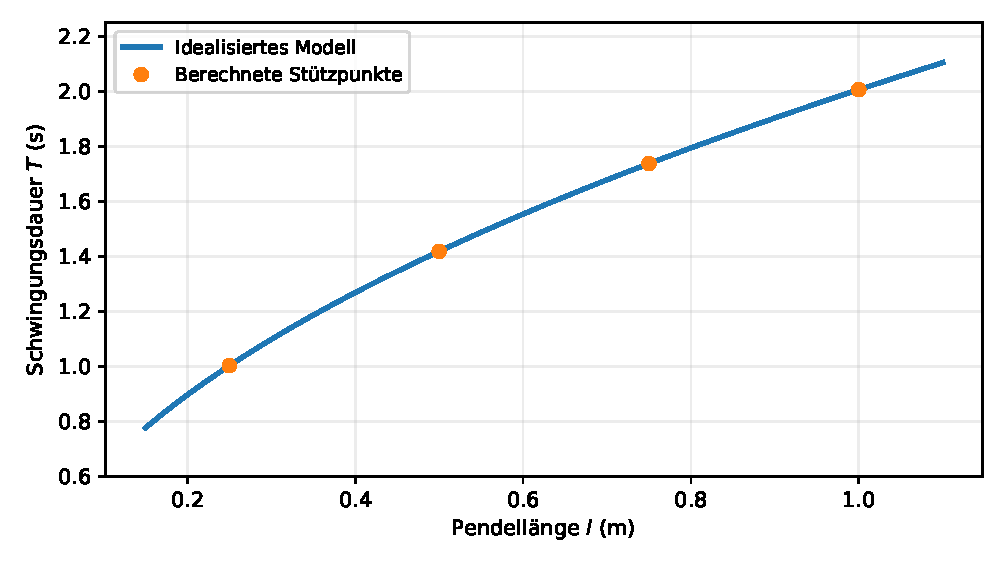
\includegraphics[width=.86\linewidth]{abbildungen/modellkurve.pdf}
  \caption{Theoretische Schwingungsdauer in Abhängigkeit von der Pendellänge
    (eigene Berechnung aus Gleichung~\eqref{eq:pendel})}
  \label{fig:modell}
\end{figure}

\chapter{Diskussion und kritische Reflexion}
\label{ch:diskussion}

\section{Einordnung der Ergebnisse}
Die Kurve in Abbildung~\ref{fig:modell} bildet den erwarteten Verlauf
des theoretischen Modells ab. Da keine Messdaten vorliegen, kann weder
die Gültigkeit des Modells experimentell überprüft noch eine
Übereinstimmung mit realen Beobachtungen behauptet werden.

\section{Grenzen, Fehlerquellen und Alternativerklärungen}
Für eine echte Messreihe wären beispielsweise eine ungenaue Bestimmung
der Pendellänge, der Startwinkel und die Zeitmessung zu berücksichtigen.
Ergebnisse müssen mit ihrer Unsicherheit und ihrem Gültigkeitsbereich
bewertet werden, nicht nur mit einer optisch passenden Kurve.

\section{Eigenanteil und Zusammenarbeit}
% Besonders wichtig bei Arbeiten, die am SFN betreut werden:
% Wer hat das Thema entwickelt, Geräte gestellt, gemessen,
% beraten, programmiert, ausgewertet oder Text korrigiert?
In einer tatsächlichen BLL wird hier transparent dokumentiert,
welche Aufgaben selbstständig ausgeführt wurden und welche Unterstützung
beispielsweise durch Lehrkräfte, SFN-Betreuende oder andere Personen
erfolgte. Das ersetzt keine vollständige Quellen- und
Hilfsmitteldokumentation.

\chapter{Fazit und Ausblick}
\label{ch:fazit}

Die Vorlage zeigt eine mögliche Struktur für eine besondere
Lernleistung. Die theoretische Beziehung \(T\propto\sqrt{l}\)
folgt aus dem idealisierten Pendelmodell. Eine experimentelle Prüfung
ist damit \emph{noch nicht} erbracht.

% In einer echten Arbeit stattdessen:
% 1) Forschungsfrage knapp beantworten,
% 2) Hauptbefunde mit Zahlen und Unsicherheiten nennen,
% 3) Grenzen der Aussage festhalten,
% 4) konkreten Ausblick formulieren.


\printbibliography[heading=bibintoc,title={Literatur- und Quellenverzeichnis}]

\appendix
\chapter{Beispiel eines Arbeits- und Messprotokolls}
\label{app:protokoll}
Die nachstehende Tabelle ist \textbf{eine leere Dokumentationshilfe},
kein Nachweis tatsächlich erbrachter Arbeit.

\begin{table}[htbp]
\centering
\caption{Vorlage für die Dokumentation des Arbeitsprozesses}
\label{tab:arbeitslog}
\begin{tabularx}{\linewidth}{@{}p{2.1cm}X p{2.6cm}@{}}
\toprule
Datum & Tätigkeit, Entscheidung, Ergebnis & Beitrag / Hilfe \\
\midrule
\rule{0pt}{2.2em} & & \\
\midrule
\rule{0pt}{2.2em} & & \\
\midrule
\rule{0pt}{2.2em} & & \\
\bottomrule
\end{tabularx}
\end{table}

% Zusätzliche Anhänge: Rohdaten, Konstruktionszeichnungen,
% Fotos des realen Aufbaus, Einverständniserklärungen,
% relevante Programmdateien oder längere Herleitungen.

% OPTIONAL: nur bei eigenem Programmcode die Zeile aktivieren:
% Optionaler Anhang. Nur aktivieren, wenn eigener Code vorhanden ist.
% Erfordert: \usepackage{listings} in gestaltung.tex
\chapter{Auswertungscode}
\lstinputlisting[language=Python,basicstyle=\ttfamily\small,
  frame=single,breaklines=true,caption={Beispielhafte Modellberechnung}]
  {code/modell.py}


\cleardoublepage
% WICHTIG: Wortlaut und Position der Erklärung vorher von der Schule
% bestätigen lassen! Eine schulische Mustererklärung geht vor.
\chapter*{Erklärung zur selbstständigen Anfertigung}
\addcontentsline{toc}{chapter}{Erklärung zur selbstständigen Anfertigung}
\thispagestyle{plain}

\textit{Hinweis: Dies ist ein Formulierungsvorschlag. Vor einer
Einreichung sind die Anforderungen der Schule einschließlich des
Umgangs mit KI-Tools und externen Hilfen zu prüfen.}

\vspace{1cm}
Ich versichere, dass ich die vorliegende Arbeit selbstständig
angefertigt und nur die angegebenen Quellen und Hilfsmittel verwendet
habe. Wörtliche und sinngemäße Übernahmen wurden kenntlich gemacht.
Fachliche, technische oder sprachliche Unterstützung durch andere
Personen und gegebenenfalls verwendete digitale Hilfsmittel habe ich
nach den Vorgaben meiner Schule offengelegt.

\vspace{.9cm}
\noindent\textbf{Dokumentation weiterer Hilfsmittel / externer Unterstützung:}\par
\vspace{.55cm}
\hrule height .3pt
\vspace{.5cm}
\hrule height .3pt

\vfill
\noindent\begin{minipage}[t]{.46\textwidth}
  \rule{\linewidth}{.4pt}\\Ort, Datum
\end{minipage}\hfill%
\begin{minipage}[t]{.46\textwidth}
  \rule{\linewidth}{.4pt}\\Unterschrift
\end{minipage}
\vspace{1.3cm}

\end{document}
